% Options for packages loaded elsewhere
\PassOptionsToPackage{unicode}{hyperref}
\PassOptionsToPackage{hyphens}{url}
\PassOptionsToPackage{dvipsnames,svgnames,x11names}{xcolor}
%
\documentclass[
  letterpaper,
  DIV=11,
  numbers=noendperiod]{scrartcl}

\usepackage{amsmath,amssymb}
\usepackage{iftex}
\ifPDFTeX
  \usepackage[T1]{fontenc}
  \usepackage[utf8]{inputenc}
  \usepackage{textcomp} % provide euro and other symbols
\else % if luatex or xetex
  \usepackage{unicode-math}
  \defaultfontfeatures{Scale=MatchLowercase}
  \defaultfontfeatures[\rmfamily]{Ligatures=TeX,Scale=1}
\fi
\usepackage{lmodern}
\ifPDFTeX\else  
    % xetex/luatex font selection
\fi
% Use upquote if available, for straight quotes in verbatim environments
\IfFileExists{upquote.sty}{\usepackage{upquote}}{}
\IfFileExists{microtype.sty}{% use microtype if available
  \usepackage[]{microtype}
  \UseMicrotypeSet[protrusion]{basicmath} % disable protrusion for tt fonts
}{}
\makeatletter
\@ifundefined{KOMAClassName}{% if non-KOMA class
  \IfFileExists{parskip.sty}{%
    \usepackage{parskip}
  }{% else
    \setlength{\parindent}{0pt}
    \setlength{\parskip}{6pt plus 2pt minus 1pt}}
}{% if KOMA class
  \KOMAoptions{parskip=half}}
\makeatother
\usepackage{xcolor}
\setlength{\emergencystretch}{3em} % prevent overfull lines
\setcounter{secnumdepth}{-\maxdimen} % remove section numbering
% Make \paragraph and \subparagraph free-standing
\ifx\paragraph\undefined\else
  \let\oldparagraph\paragraph
  \renewcommand{\paragraph}[1]{\oldparagraph{#1}\mbox{}}
\fi
\ifx\subparagraph\undefined\else
  \let\oldsubparagraph\subparagraph
  \renewcommand{\subparagraph}[1]{\oldsubparagraph{#1}\mbox{}}
\fi


\providecommand{\tightlist}{%
  \setlength{\itemsep}{0pt}\setlength{\parskip}{0pt}}\usepackage{longtable,booktabs,array}
\usepackage{calc} % for calculating minipage widths
% Correct order of tables after \paragraph or \subparagraph
\usepackage{etoolbox}
\makeatletter
\patchcmd\longtable{\par}{\if@noskipsec\mbox{}\fi\par}{}{}
\makeatother
% Allow footnotes in longtable head/foot
\IfFileExists{footnotehyper.sty}{\usepackage{footnotehyper}}{\usepackage{footnote}}
\makesavenoteenv{longtable}
\usepackage{graphicx}
\makeatletter
\def\maxwidth{\ifdim\Gin@nat@width>\linewidth\linewidth\else\Gin@nat@width\fi}
\def\maxheight{\ifdim\Gin@nat@height>\textheight\textheight\else\Gin@nat@height\fi}
\makeatother
% Scale images if necessary, so that they will not overflow the page
% margins by default, and it is still possible to overwrite the defaults
% using explicit options in \includegraphics[width, height, ...]{}
\setkeys{Gin}{width=\maxwidth,height=\maxheight,keepaspectratio}
% Set default figure placement to htbp
\makeatletter
\def\fps@figure{htbp}
\makeatother

\KOMAoption{captions}{tableheading}
\makeatletter
\@ifpackageloaded{caption}{}{\usepackage{caption}}
\AtBeginDocument{%
\ifdefined\contentsname
  \renewcommand*\contentsname{Table of contents}
\else
  \newcommand\contentsname{Table of contents}
\fi
\ifdefined\listfigurename
  \renewcommand*\listfigurename{List of Figures}
\else
  \newcommand\listfigurename{List of Figures}
\fi
\ifdefined\listtablename
  \renewcommand*\listtablename{List of Tables}
\else
  \newcommand\listtablename{List of Tables}
\fi
\ifdefined\figurename
  \renewcommand*\figurename{Figure}
\else
  \newcommand\figurename{Figure}
\fi
\ifdefined\tablename
  \renewcommand*\tablename{Table}
\else
  \newcommand\tablename{Table}
\fi
}
\@ifpackageloaded{float}{}{\usepackage{float}}
\floatstyle{ruled}
\@ifundefined{c@chapter}{\newfloat{codelisting}{h}{lop}}{\newfloat{codelisting}{h}{lop}[chapter]}
\floatname{codelisting}{Listing}
\newcommand*\listoflistings{\listof{codelisting}{List of Listings}}
\makeatother
\makeatletter
\makeatother
\makeatletter
\@ifpackageloaded{caption}{}{\usepackage{caption}}
\@ifpackageloaded{subcaption}{}{\usepackage{subcaption}}
\makeatother
\ifLuaTeX
  \usepackage{selnolig}  % disable illegal ligatures
\fi
\usepackage{bookmark}

\IfFileExists{xurl.sty}{\usepackage{xurl}}{} % add URL line breaks if available
\urlstyle{same} % disable monospaced font for URLs
\hypersetup{
  pdftitle={Analysis of the health of Montgomery County, Maryland},
  pdfauthor={Mychala Walker},
  colorlinks=true,
  linkcolor={blue},
  filecolor={Maroon},
  citecolor={Blue},
  urlcolor={Blue},
  pdfcreator={LaTeX via pandoc}}

\title{Analysis of the health of Montgomery County, Maryland}
\usepackage{etoolbox}
\makeatletter
\providecommand{\subtitle}[1]{% add subtitle to \maketitle
  \apptocmd{\@title}{\par {\large #1 \par}}{}{}
}
\makeatother
\subtitle{Based on Social Determinants of Health from the U.S. Dept. of
Health and Human Services}
\author{Mychala Walker}
\date{}

\begin{document}
\maketitle

\subsection{Introduction}\label{introduction}

For this paper, I intend to accomplish two things: 1) determine the
overall health of Montgomery County, Maryland and 2) compare the health
status of the different Census tracts of Montgomery County, Maryland. I
employ the U.S. Department of Health and Human Services' five (5) social
determinant groups of health. The social determinant groups are economic
stability, education access and quality, health care access and quality,
neighborhood and built environment, \& social and community context.
Within these groups are a number of variables which will be explained in
great detail below. To compare the tracts, I will create eight (8)
k-means clusters of the Census tracts and analyze the clusters, both
demographically and based on the social determinants of health factors.
The total within sum of square method was used to determine the optimal
number of clusters for this model.

\subsection{Data}\label{data}

For this study, I combine multiple datasets from two sources: 1) the
2022 U.S. American Community Survey (ACS) and 2) Montgomery County,
Maryland Open Data Portal. The combined data set had 232 observations
where every observation is a census tract. Census tracts are small,
relatively permanent statistical subdivisions of the County from the
U.S. Census Bureau. According to the the U.S. Census Bureau, each area
contains approximately 4,000 people of relatively homogeneous
characteristics with respect to population, economic status and living
conditions. Census tracts provide a stable set of geographic units for
the presentation of decennial census data over the decades and are only
occasionally split to reflect population growth. The model estimated
that eight (8) clusters was optimal using the the total within sum of
squares method.

The dataset had 42 variables that represent both demographic and social
determinants of health based on standards set by U.S. Human and Health
Services. According to the U.S. Human and Health Services, social
determinants of health (SDOH) are the conditions in the environments
where people are born, live, learn, work, play, worship, and age that
affect a wide range of health, functioning, and quality-of-life outcomes
and risks. Social determinants of health also contribute to wide health
disparities and inequities. Variables on employment, number of grocery
stores, housing insecurity, and poverty are used to represent economic
stability. Variables on early childhood development and poverty,
enrollment in higher education, high school graduation are used to
represent education access and quality. Variables on the number of HHS
facilities are used to represent health care access and quality.
Variables on number of grocery stores, amount of crimes, and
neighborhood walk score are used to represent neighborhood and built
environment. There were no variables used to represent social and
community context. All of the variables are numeric variables except for
the GEOID variable. There is also a geometry variable for graphing
purposes.

\subsection{Analysis}\label{analysis}

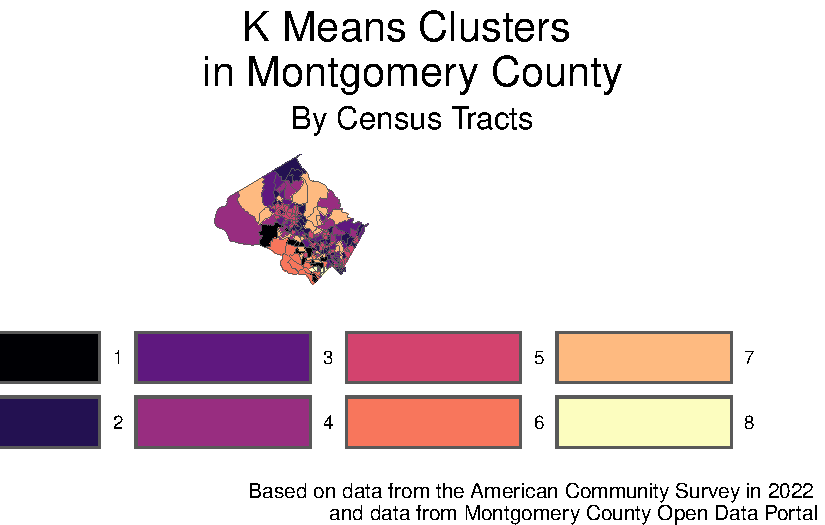
\includegraphics{final_project_files/figure-pdf/graphs-1.pdf}

As we can see from the above graphs, the are a few clusters that seem to
be sectioned to one part of the county. For example, clusters one (1),
six (6), and eight (8) seems to only be in the bottom part of the
county. Further, cluster five (5) seems to be portioned mostly in the
center part of the county. The mean demographics of the clusters
themselves are interesting.

\begin{verbatim}
# A tibble: 8 x 7
  cluster mean_pop mean_whipop mean_blkpop mean_hispop mean_income mean_age
*   <int>    <dbl>       <dbl>       <dbl>       <dbl>       <dbl>    <dbl>
1       1    4441.        69.6        4.63        7.55     287558.     45.3
2       2    4814.        44.5       19.4        22.4      138586.     39.0
3       3    4743.        47.4       17.2        18.0      169925.     40.9
4       4    4617.        55.7       13.0        11.4      197021.     43.4
5       5    4461.        31.1       28.7        30.0      101300.     37.8
6       6    4725.        69.8        5.12        6.78     357641.     48.1
7       7    4262.        63.0        9.15        9.48     224252.     45.0
8       8    3302.        82.3        2           4.7      492099.     49.6
\end{verbatim}

Cluster 8 has a significantly high white population, high mean income,
high mean life expectancy and low poverty. On the other hand, cluster 5
has a significantly high minority population, high unemployment, high
poverty, and low life expectancy. Clusters 1, 6, and 7 are on the high
end for white population and low minority population. Unemployment rate
is similar across the clusters, with the exception of clusters 5 and 8,
the unemployment rate are around 3 and 4. The mean income across the
clusters range from \$101,000 and \$493,000. The average age is also
pretty similar across all the clusters with a range of 37 and 49 years
old. Interestingly, cluster 5 is the ``youngest'' cluster whereas
cluster 8 is the ``oldest''.

\begin{verbatim}
# A tibble: 8 x 11
  cluster mean_travelwrk own_rent_rto mean_unigrad mean_schoolenroll
*   <int>          <dbl>        <dbl>        <dbl>             <dbl>
1       1           31.1        6.26         2542.             1246 
2       2           33.1        1.78         1893.             1163.
3       3           32.6        2.80         1916.             1246.
4       4           34.2        5.16         2221.             1196.
5       5           33.0        0.751        1292.             1090.
6       6           30.0        9.18         2874.             1259.
7       7           33.2        7.78         2158.             1133.
8       8           29.3       11.8          2148.              871.
# i 6 more variables: mean_noinsure <dbl>, mean_unemploy <dbl>,
#   mean_violent <dbl>, mean_poverty <dbl>, mean_lifeexpectancy <dbl>,
#   mean_grocery <dbl>
\end{verbatim}

As for the social determinants of health, we see a similar trend.
Cluster 8 is an all around wealthy and healthy cluster. Their own to
rent ratio is significantly higher than than the other clusters. Their
population with no insurance is low and their number of violent crimes
is low. As for cluster 5, we see the complete opposite. Their
no-insurance population is the highest amongst all of the clusters.
There violent crime rate is also extremely high compared to the other
clusters. Based on these findings and the standards set by HHS, this
cluster would be deemed unhealthy. Interestingly, amongst all of the
clusters, the university graduate population rate is similar. The own to
rent ratio between the clusters are also starkingly different. With the
exception of cluster eight (8), child age school enrollment is similar.

\subsection{Conclusion}\label{conclusion}

Based on these findings and the standards set by HHS, comparatively,
clusters 1, 6, 7, and 8 are the healthiest clusters in Montgomery
county. On the other side, clusters 2, 3, 4, and 5 are the least
healthy. This means that representatives and local officials from
representing clusters 2, 3, 4, and 5 to consider programming that may
improve social conditions, with the goal of improving health outcomes.



\end{document}
